\documentclass[twoside,10pt]{article}

\usepackage{blindtext}

% Any additional packages needed should be included after jmlr2e.
% Note that jmlr2e.sty includes epsfig, amssymb, natbib and graphicx,
% and defines many common macros, such as 'proof' and 'example'.
%
% It also sets the bibliographystyle to plainnat; for more information on
% natbib citation styles, see the natbib documentation, a copy of which
% is archived at http://www.jmlr.org/format/natbib.pdf

% Available options for package jmlr2e are:
%
%   - abbrvbib : use abbrvnat for the bibliography style
%   - nohyperref : do not load the hyperref package
%   - preprint : remove JMLR specific information from the template,
%         useful for example for posting to preprint servers.
%
% Example of using the package with custom options:
%
% \usepackage[abbrvbib, preprint]{jmlr2e}

\usepackage{jmlr2e}
\graphicspath{{media/}} 
% Definitions of handy macros can go here

\newcommand{\dataset}{{\cal D}}
\newcommand{\fracpartial}[2]{\frac{\partial #1}{\partial  #2}}

% Heading arguments are {volume}{year}{pages}{date submitted}{date published}{paper id}{author-full-names}

\usepackage{lastpage}
\jmlrheading{23}{2022}{1-\pageref{LastPage}}{1/21; Revised 5/22}{9/22}{21-0000}{Author One and Author Two}

% Short headings should be running head and authors last names

\ShortHeadings{Sample JMLR Paper}{One and Two}
\firstpageno{1}

\begin{document}

\title{Sample JMLR Paper}

\author{\name Author One \email one@stat.washington.edu \\
       \addr Department of Statistics\\
       University of Washington\\
       Seattle, WA 98195-4322, USA
       \AND
       \name Author Two \email two@cs.berkeley.edu \\
       \addr Division of Computer Science\\
       University of California\\
       Berkeley, CA 94720-1776, USA}

\editor{My editor}

\begin{figure}[htb]
  \centering
  \newcommand{\imgwidth}{0.22\textwidth}

  % first row: images 1–4 with n values
  \begin{subfigure}[b]{\imgwidth}
    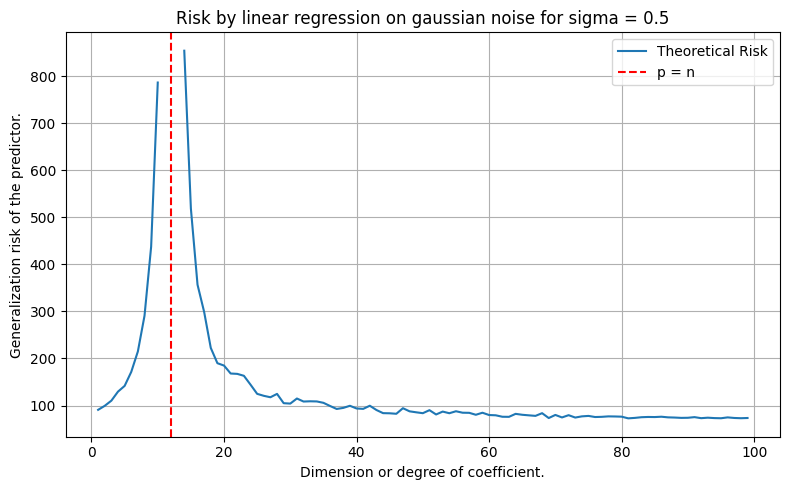
\includegraphics[width=\linewidth]{img/descent_lin_reg_1.png}
    \caption{$n=12$}\label{fig:1a}
  \end{subfigure}%
  \hfill
  \begin{subfigure}[b]{\imgwidth}
    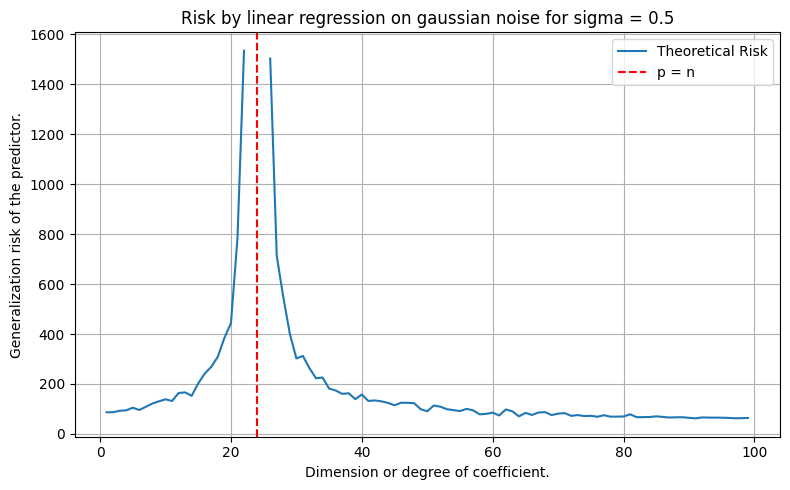
\includegraphics[width=\linewidth]{img/descent_lin_reg_2.png}
    \caption{$n=24$}\label{fig:1b}
  \end{subfigure}%
  \hfill
  \begin{subfigure}[b]{\imgwidth}
    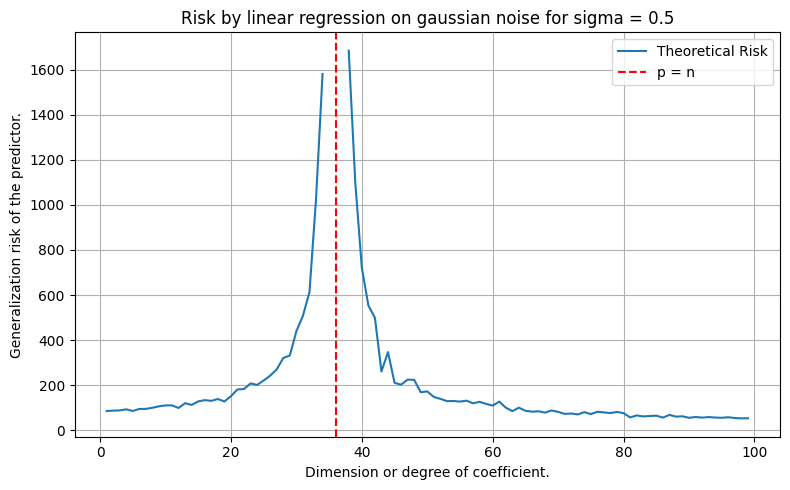
\includegraphics[width=\linewidth]{img/descent_lin_reg_3.png}
    \caption{$n=36$}\label{fig:1c}
  \end{subfigure}%
  \hfill
  \begin{subfigure}[b]{\imgwidth}
    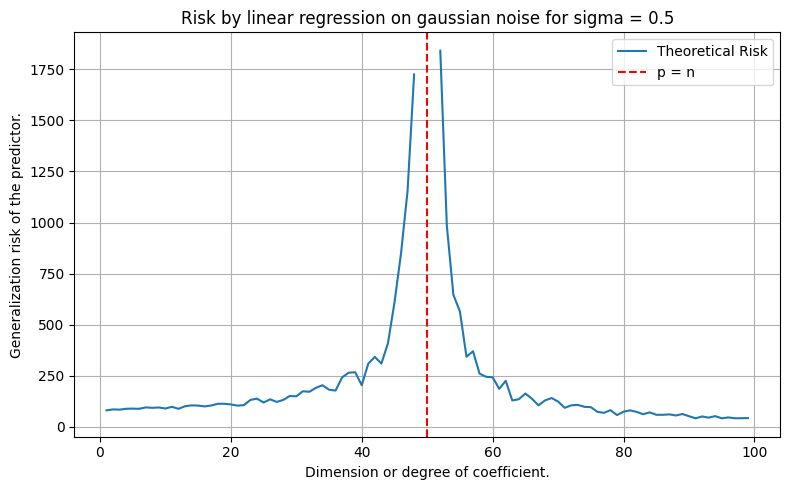
\includegraphics[width=\linewidth]{img/descent_lin_reg_4.png}
    \caption{$n=50$}\label{fig:1d}
  \end{subfigure}

  \medskip

  % second row: images 5–8 with n values
  \begin{subfigure}[b]{\imgwidth}
    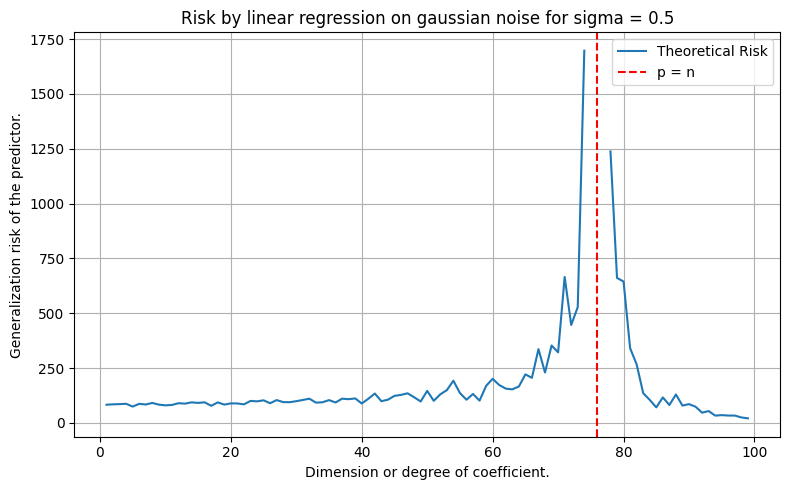
\includegraphics[width=\linewidth]{img/descent_lin_reg_5.png}
    \caption{$n=76$}\label{fig:2a}
  \end{subfigure}%
  \hfill
  \begin{subfigure}[b]{\imgwidth}
    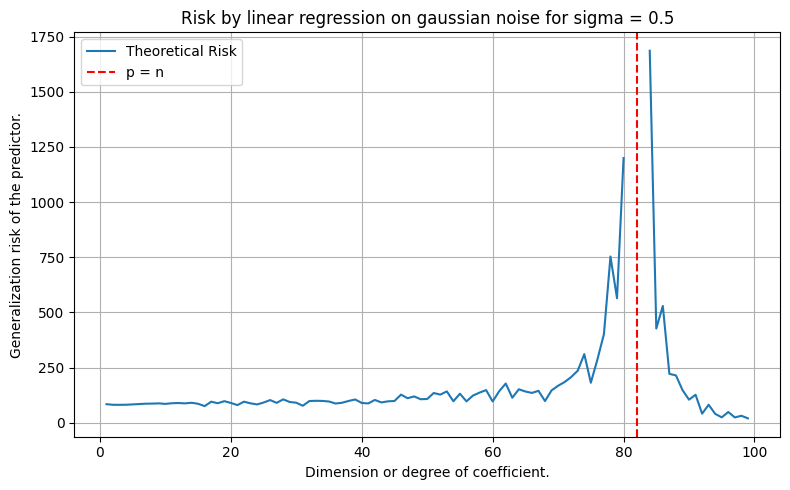
\includegraphics[width=\linewidth]{img/descent_lin_reg_6.png}
    \caption{$n=82$}\label{fig:2b}
  \end{subfigure}%
  \hfill
  \begin{subfigure}[b]{\imgwidth}
    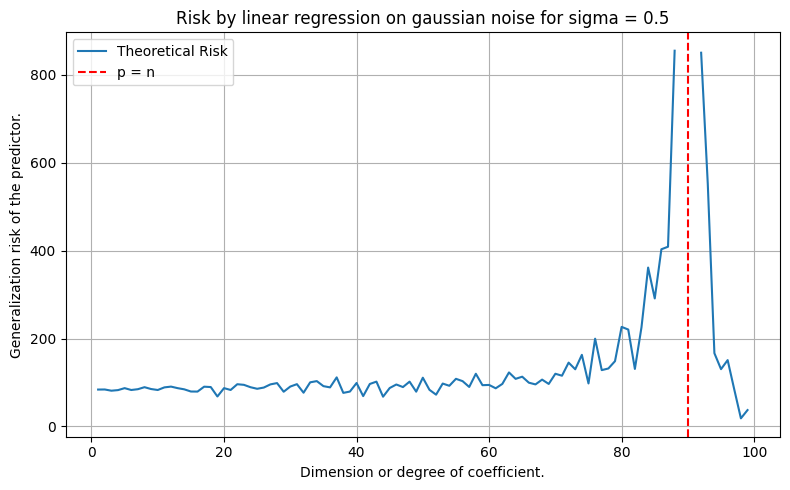
\includegraphics[width=\linewidth]{img/descent_lin_reg_7.png}
    \caption{$n=90$}\label{fig:2c}
  \end{subfigure}%
  \hfill
  \begin{subfigure}[b]{\imgwidth}
    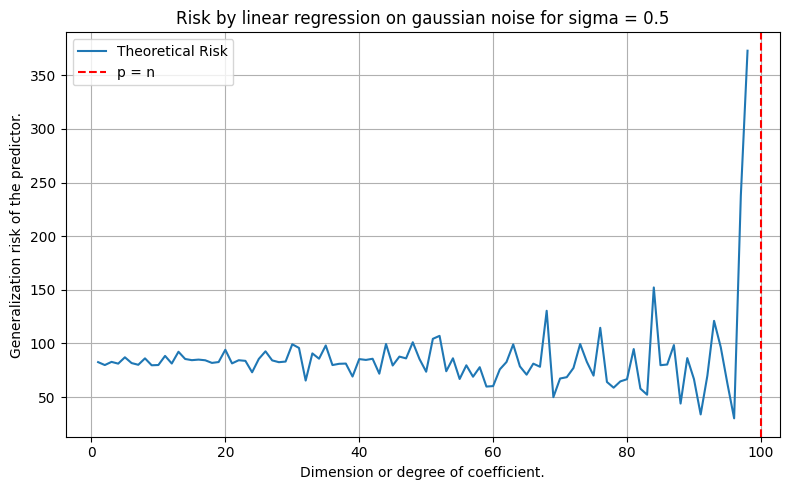
\includegraphics[width=\linewidth]{img/descent_lin_reg_8.png}
    \caption{$n=100$}\label{fig:2d}
  \end{subfigure}

  \medskip

  % third row: images 9–11 with n values
  \begin{subfigure}[b]{\imgwidth}
    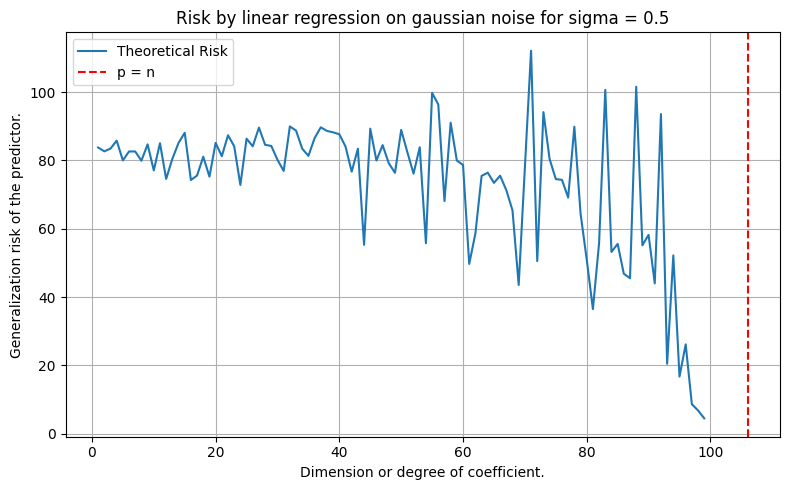
\includegraphics[width=\linewidth]{img/descent_lin_reg_9.png}
    \caption{$n=106$}\label{fig:3a}
  \end{subfigure}%
  \hfill
  \begin{subfigure}[b]{\imgwidth}
    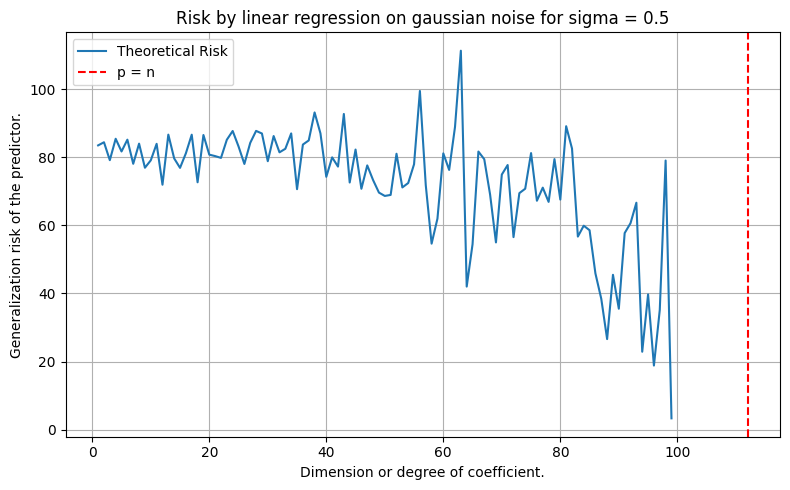
\includegraphics[width=\linewidth]{img/descent_lin_reg_10.png}
    \caption{$n=112$}\label{fig:3b}
  \end{subfigure}%
  \hfill
  \begin{subfigure}[b]{\imgwidth}
    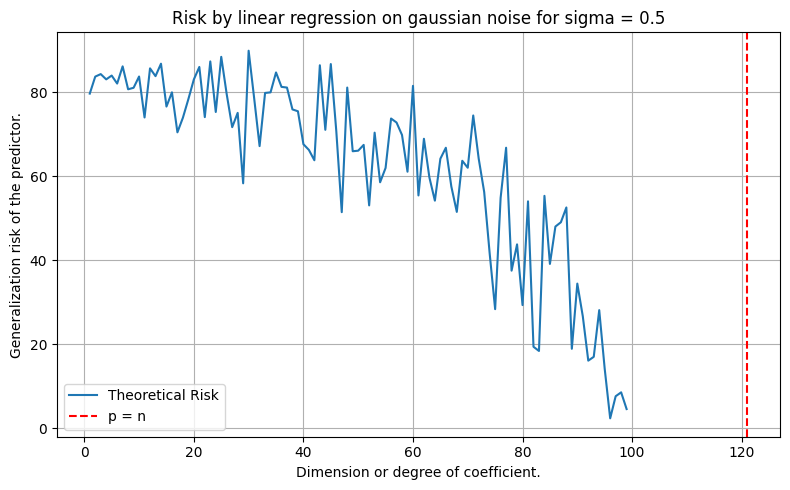
\includegraphics[width=\linewidth]{img/descent_lin_reg_11.png}
    \caption{$n=121$}\label{fig:3c}
  \end{subfigure}%
  \hfill
  \begin{subfigure}[b]{\imgwidth}
    ~
  \end{subfigure}

  \caption{Theorem~\ref{thm:double_descent_lr} behaviours on randomized setting. For this model, we have $d=100$, $\sigma = 0.5$, and variational $n$. Full test cases are for $p=[1,100]$, $n=\{12,24,36,50,76,82,90,100,106,112,121\}$ accordingly. The test function of the concept itself is the same linear model, but with different input only.}
  \label{fig:11grid}
\end{figure}

\begin{figure}[htb]
  \centering
  \newcommand{\imgwidth}{0.22\textwidth}

  % first row: images 1–4 with n values
  \begin{subfigure}[b]{\imgwidth}
    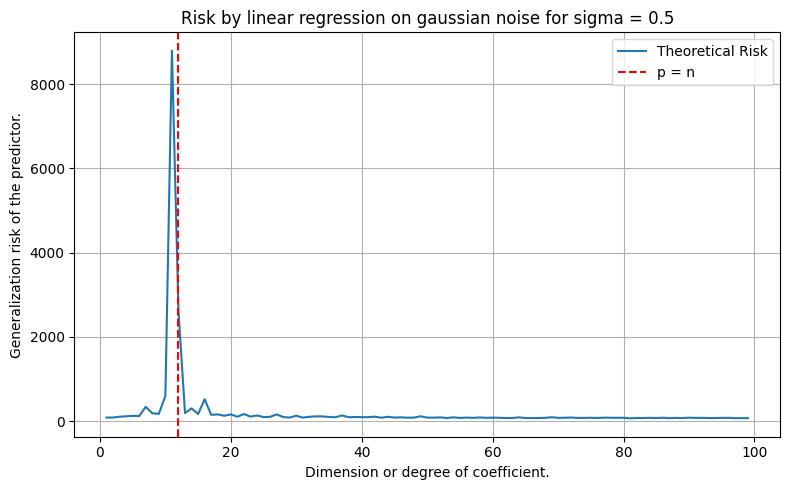
\includegraphics[width=\linewidth]{img/descent_devel1.png}
    \caption{$n=12$}\label{fig:1a2}
  \end{subfigure}%
  \hfill
  \begin{subfigure}[b]{\imgwidth}
    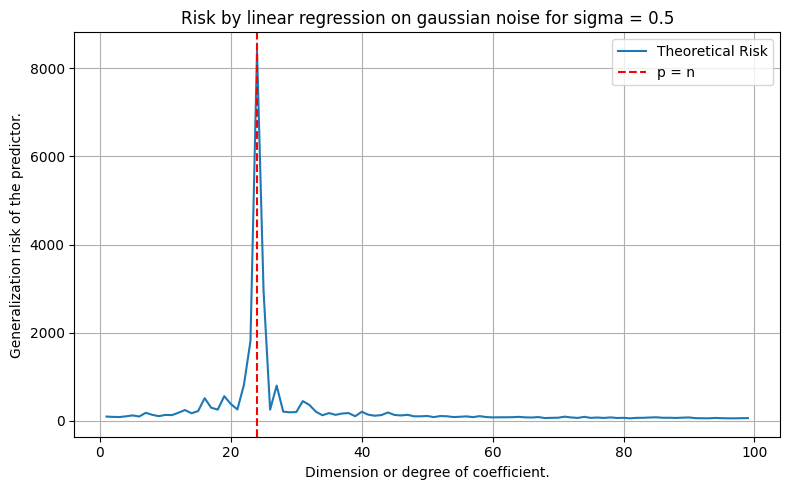
\includegraphics[width=\linewidth]{img/descent_devel2.png}
    \caption{$n=24$}\label{fig:1b2}
  \end{subfigure}%
  \hfill
  \begin{subfigure}[b]{\imgwidth}
    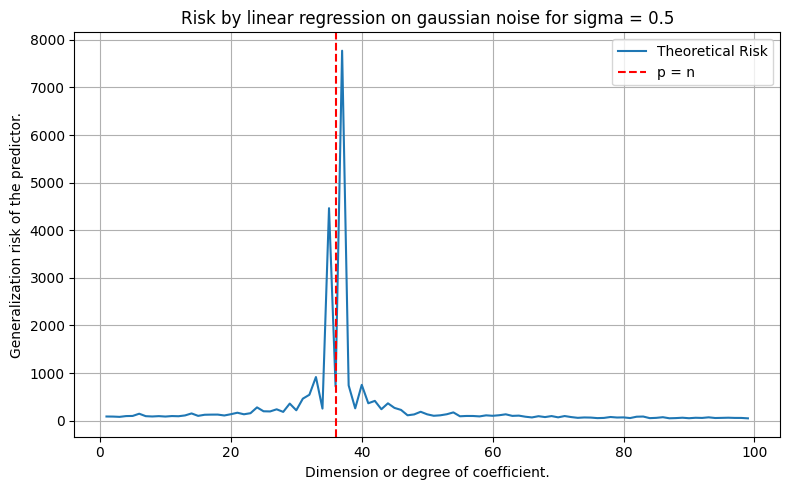
\includegraphics[width=\linewidth]{img/descent_devel3.png}
    \caption{$n=36$}\label{fig:1c2}
  \end{subfigure}%
  \hfill
  \begin{subfigure}[b]{\imgwidth}
    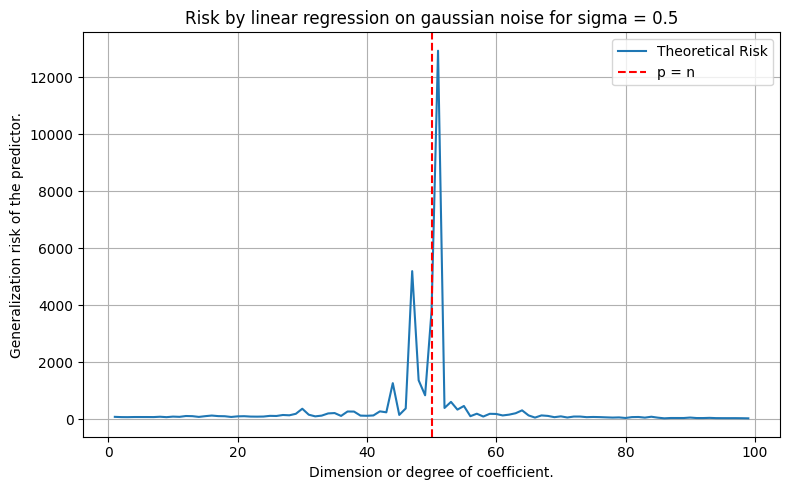
\includegraphics[width=\linewidth]{img/descent_devel4.png}
    \caption{$n=50$}\label{fig:1d2}
  \end{subfigure}

  \medskip

  % second row: images 5–8 with n values
  \begin{subfigure}[b]{\imgwidth}
    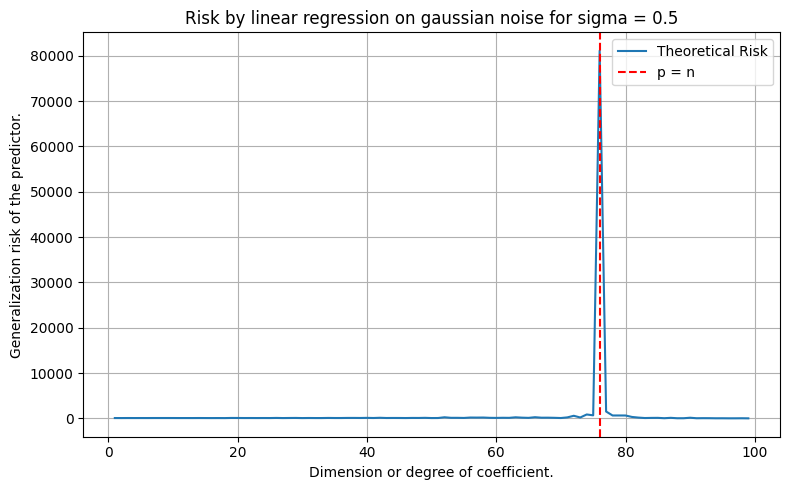
\includegraphics[width=\linewidth]{img/descent_devel5.png}
    \caption{$n=76$}\label{fig:2a2}
  \end{subfigure}%
  \hfill
  \begin{subfigure}[b]{\imgwidth}
    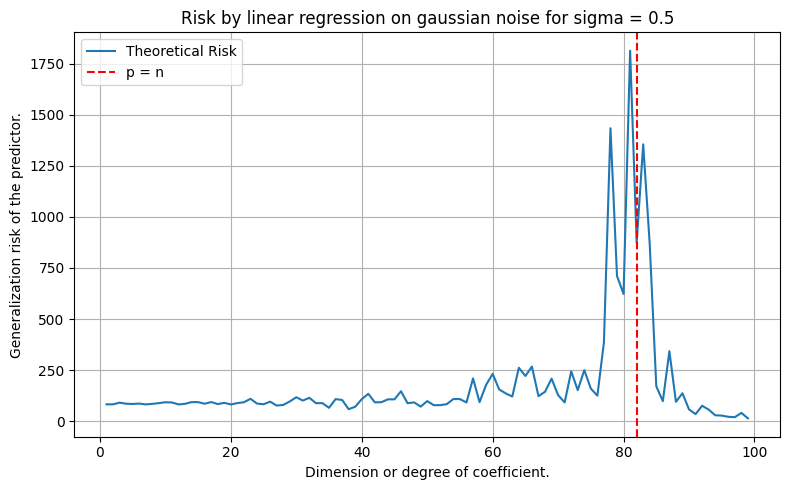
\includegraphics[width=\linewidth]{img/descent_devel6.png}
    \caption{$n=82$}\label{fig:2b2}
  \end{subfigure}%
  \hfill
  \begin{subfigure}[b]{\imgwidth}
    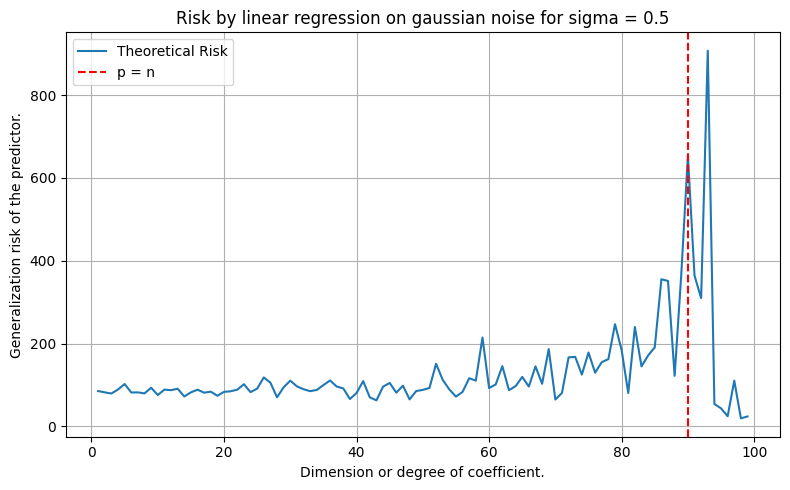
\includegraphics[width=\linewidth]{img/descent_devel7.png}
    \caption{$n=90$}\label{fig:2c2}
  \end{subfigure}%
  \hfill
  \begin{subfigure}[b]{\imgwidth}
    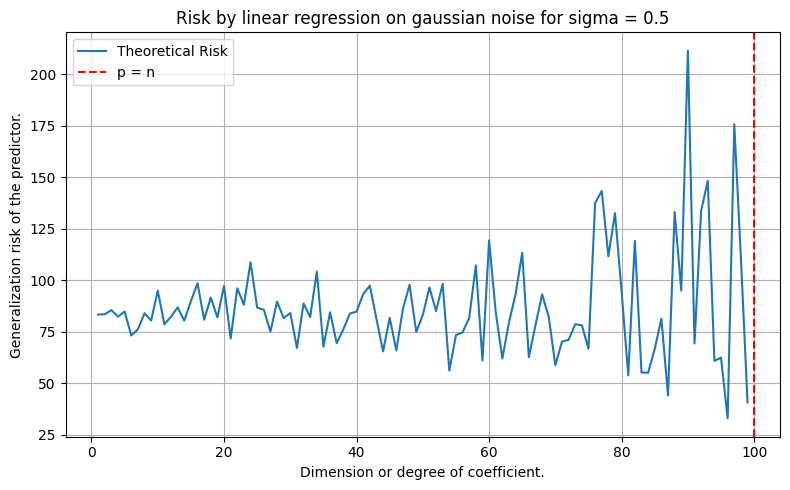
\includegraphics[width=\linewidth]{img/descent_devel8.png}
    \caption{$n=100$}\label{fig:2d2}
  \end{subfigure}

  \medskip

  % third row: images 9–11 with n values
  \begin{subfigure}[b]{\imgwidth}
    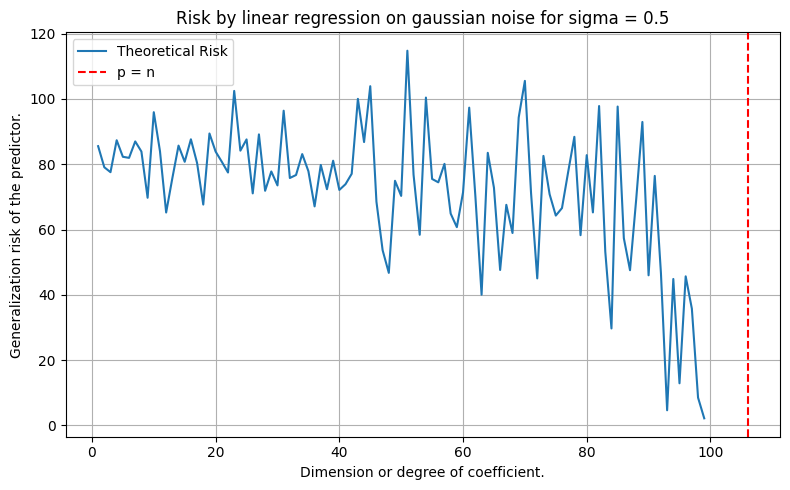
\includegraphics[width=\linewidth]{img/descent_devel9.png}
    \caption{$n=106$}\label{fig:3a2}
  \end{subfigure}%
  \hfill
  \begin{subfigure}[b]{\imgwidth}
    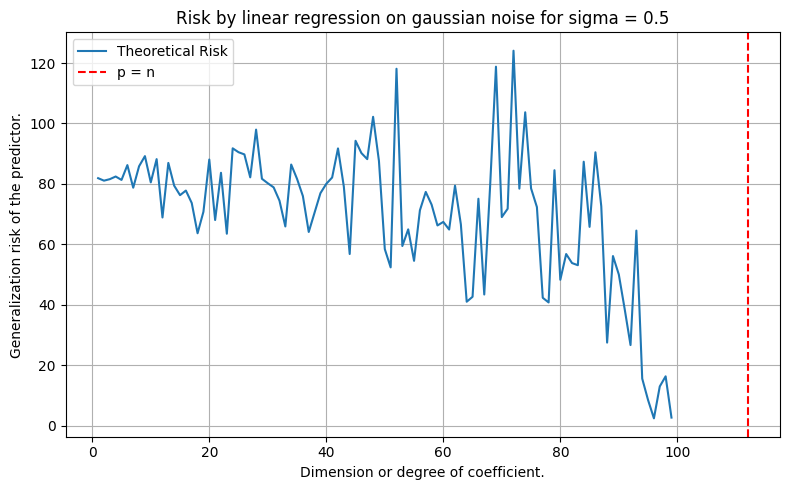
\includegraphics[width=\linewidth]{img/descent_devel10.png}
    \caption{$n=112$}\label{fig:3b2}
  \end{subfigure}%
  \hfill
  \begin{subfigure}[b]{\imgwidth}
    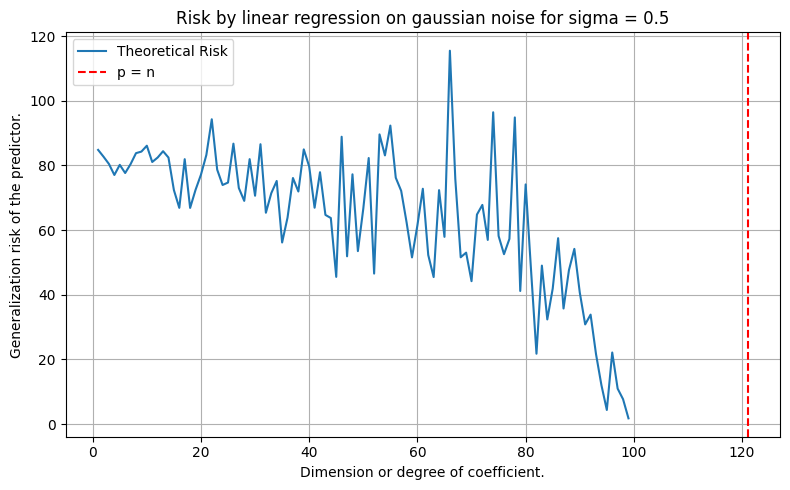
\includegraphics[width=\linewidth]{img/descent_devel11.png}
    \caption{$n=121$}\label{fig:3c2}
  \end{subfigure}%
  \hfill
  \begin{subfigure}[b]{\imgwidth}
    ~
  \end{subfigure}

  \caption{Contrary to Theorem~\ref{thm:double_descent_lr}, this is the behaviours on randomized setting for standard parameter-wised mean square error measure (MSE-on-parameter). For this model, we have $d=100$, $\sigma = 0.5$, and variational $n$. Full test cases are for $p=[1,100]$, $n=\{12,24,36,50,76,82,90,100,106,112,121\}$ accordingly. The test function of the concept itself is the same linear model, but with different input only.}
  \label{fig:11grid2}
\end{figure}
\end{document}
